% !TEX program = pdflatex
\documentclass{article}

\usepackage{PRIMEarxiv}
\usepackage[utf8]{inputenc}
\usepackage[T1]{fontenc}
\usepackage{hyperref}
\usepackage{url}
\usepackage{booktabs}
\usepackage{amsfonts}
\usepackage{nicefrac}
\usepackage{microtype}
\usepackage{fancyhdr}
\usepackage{graphicx}
\usepackage{enumitem}
\graphicspath{{./}{plots/}{ablation_study/reports/}}
\usepackage{float}
% Header
\pagestyle{fancy}
\thispagestyle{empty}
\rhead{ \textit{ }}
\fancyhead[LO]{Antimicrobial Activity Prediction}

% Title
\title{Predicting Antimicrobial Activity of Peptides Against Specific Bacteria Using Machine Learning}

\author{Yann Baglin-Bunod \\
UC San Diego \\
\texttt{ybaglinbunod@ucsd.edu}}

\begin{document}
\maketitle

\begin{abstract}
I present a dual-sequence predictor of antimicrobial activity that takes a bacterial DNA segment and a peptide amino acid sequence as inputs and outputs a probability score indicating whether the peptide is likely to kill the bacterium. This project also investigates how Claude, an AI assistant, can be leveraged to accelerate code development for machine learning research. I describe the dataset, the Claude-generated baseline with a training/evaluation pipeline, and a multi-seed 70/15/15 split ablation study (ROC/PR, calibration, threshold sweeps). I report accuracy/ROC-AUC (mean~$\pm$~std) across seeds and release artifacts for reproducibility.
\end{abstract}


\section{Introduction / Background}
Antimicrobial peptides (AMPs) are molecules that play a central role in the innate immune system by targeting and disrupting microbial cell membranes. They are increasingly studied as promising alternatives to conventional antibiotics, especially in the context of rising antimicrobial resistance. Predicting the activity of a peptide against a specific bacterium is a challenging task that traditionally requires expensive and time-consuming laboratory assays. Machine learning models offer the possibility of accelerating this process by leveraging sequence data to make rapid, scalable predictions.

At the same time, AI coding assistants such as Claude are beginning to transform how researchers build and iterate on machine learning pipelines. They provide fast generation of boilerplate code, offer debugging suggestions, and can accelerate the experimental cycle. However, their outputs still require careful oversight and domain expertise to ensure scientific rigor. This paper explores both the biological modeling challenge and the methodological question of how Claude can be effectively used as a tool for machine learning research.

\section{Dataset Development}
The dataset for this project was curated and provided by Nam Do. I worked with the \texttt{train\_sequence.json} file, which contains peptide sequences paired with bacterial DNA segments and associated binary activity labels. This file had already been preprocessed into a format suitable for model training, ensuring consistency across inputs and outputs. It was used for both predictor development and evaluation experiments.

The underlying data was assembled from DRAMP and related resources. It was consolidated information from multiple spreadsheets, including \texttt{general\_amps.xlsx} (11,613 entries), \texttt{clinical\_amps.xlsx}, \texttt{specific\_amps.xlsx}, \texttt{expanded\_amps.xlsx}, \texttt{stability\_amps.xlsx}, and \texttt{patent\_amps.xlsx}, which collectively provide peptide sequences, names, reported activities, structures, target organisms, and references. To standardize inputs, target organism names were cleaned to remove aliases, and representative genomes were retrieved from NCBI using the \texttt{datasets} CLI to build DNA context. 
\section{Methods / Architecture}

The baseline model was first generated with Claude and then modified into a usable PyTorch script (\textbf{\texttt{antimicrobial\_predictor.py}}). For preprocessing, sequences are integer-tokenized and truncated or padded to fixed lengths (50 nucleotides for DNA and 100 amino acids for peptides). The architecture was first generated by Claude, then modified by me. It consists of two branches: a DNA branch that applies an embedding layer, a convolutional neural network, and adaptive max pooling, and a peptide branch that applies an embedding layer, a two-layer bidirectional LSTM, an eight-head self-attention mechanism, and a masked global average pool (Figure~\ref{fig:media/model_overview.png}). The resulting feature representations are concatenated and passed through a multilayer perceptron classifier (MLP) with dropout and a sigmoid activation.  

Training uses Adam (learning rate $1\times10^{-3}$), binary cross-entropy loss, weight decay $1\times10^{-5}$, gradient clipping, ReduceLROnPlateau scheduling, and early stopping. The best model according to validation accuracy is versioned, while per-epoch checkpoints are stored under \texttt{ablation\_study/runs/}.

\begin{figure}[htbp]
  \centering
  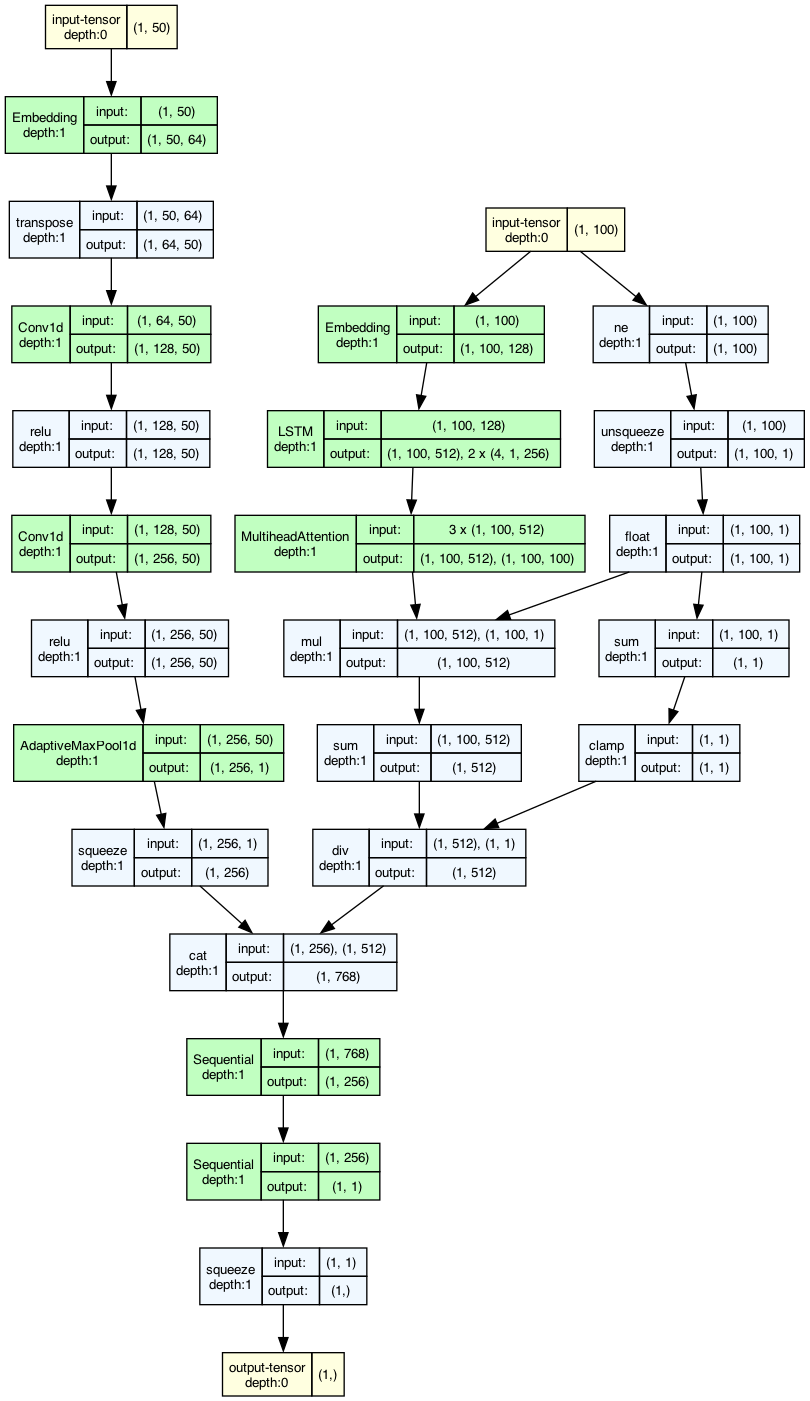
\includegraphics[width=.5\linewidth]{media/model_overview.png}
  \caption{level model overview (DNA branch, peptide branch, fusion, classifier).}
\end{figure}

\section{Results and Ablation Study}
Initial validation experiments showed strong accuracy and ROC-AUC performance on the held-out validation set. We observed limitations with Claude’s code generation, as it occasionally proposed synthetic placeholder data in the absence of real inputs. To avoid misleading results, these were replaced with curated CSVs granted by Nam Do. Diagnostic checks including learning curves and sample predictions confirmed stable training behavior (see training history and model overview figures).

\begin{figure}[H]
  \centering
  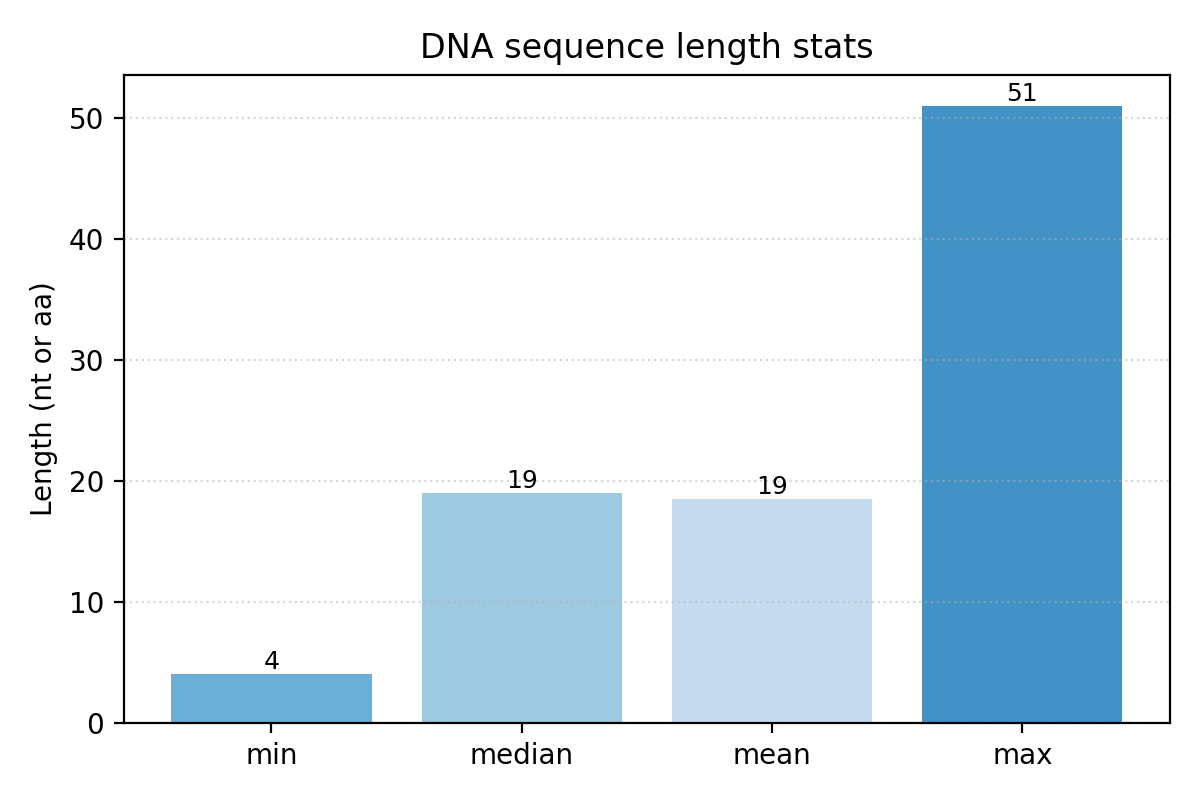
\includegraphics[width=.45\linewidth]{media/dna_length_stats.png}
  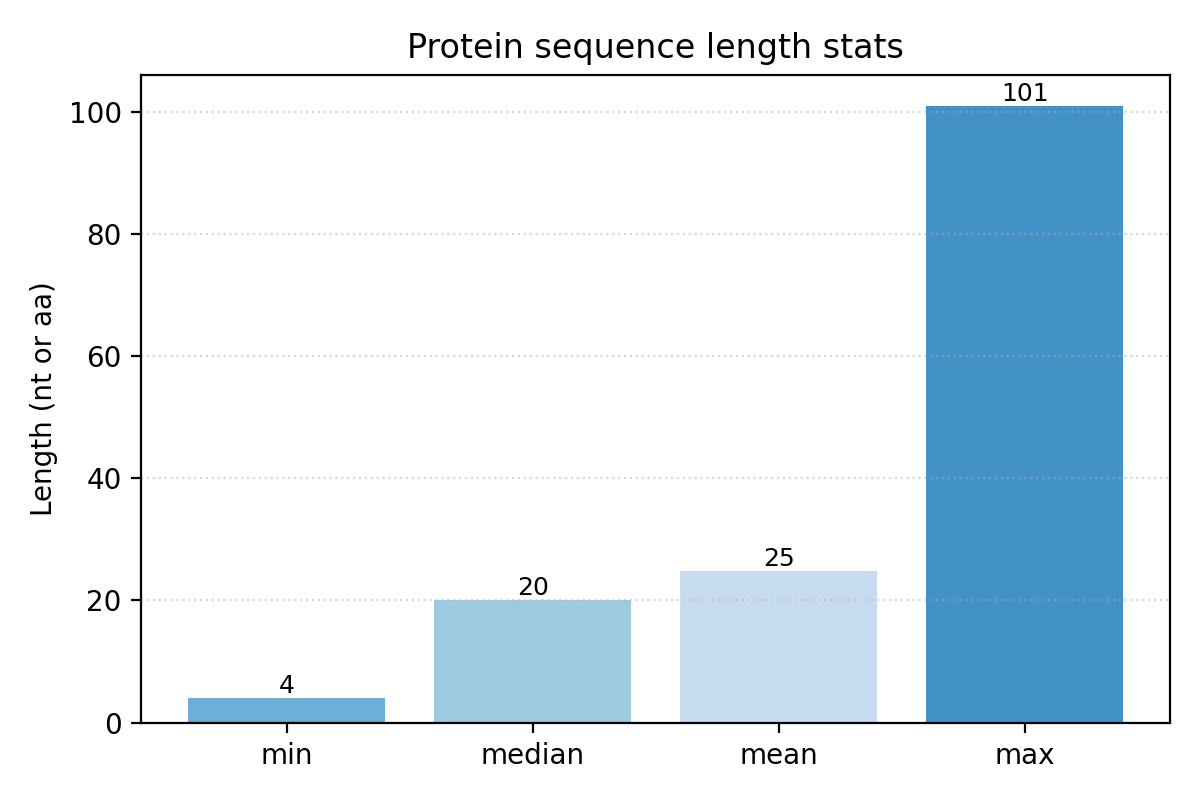
\includegraphics[width=.45\linewidth]{media/protein_length_stats.png}
  \caption{Sequence length summaries (DNA and peptide).}
\end{figure}

\noindent The threshold sweep (Figure~\ref{fig:thresh}) summarizes precision/recall trade-offs across operating points: we see that a threshold of 0.42 yields the highest F1 score as seen in the figure.

\begin{figure}[H]
  \centering
  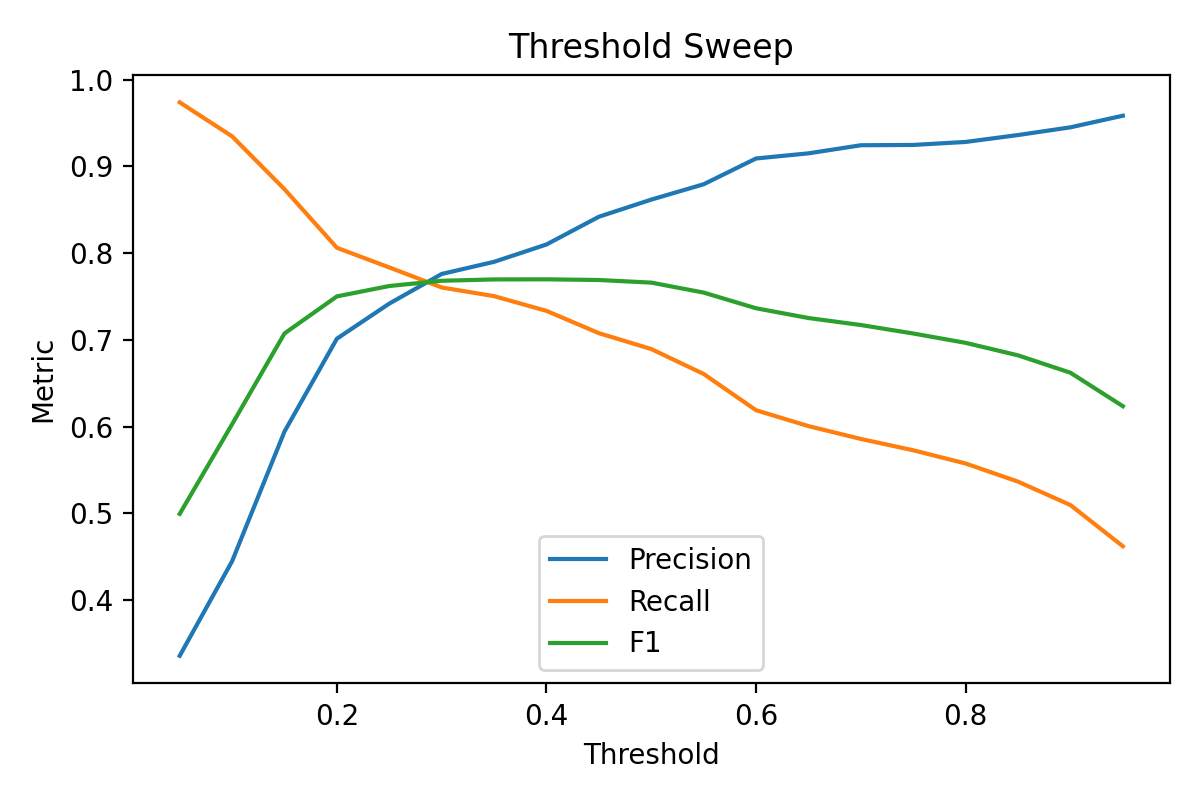
\includegraphics[width=.6\linewidth]{threshold_sweep.png}
  \caption{Precision, recall, and F1 versus decision threshold on a representative seed.}
  \label{fig:thresh}
\end{figure}

To evaluate the model, I adopted a 70/15/15 train/validation/test split with five different random seeds. For each seed, I measured test accuracy and ROC-AUC, reporting the mean and standard deviation across runs. In addition, I generated ROC and PR curves, calibration plots, threshold sweeps, confusion matrices, score distributions, and analyses of sequence length effects. These outputs are included in \texttt{ablation\_study/reports/}, providing a comprehensive picture of the model’s strengths and weaknesses under different evaluation settings. We can see from table~\ref{tab:summary} that the model achieves both high predictive performance and remarkable stability across random initializations, giving confidence that the reported accuracy are robust rather than seed-dependent.

\noindent Example figures (update date/seed as needed):
\begin{figure}[H]
  \centering
  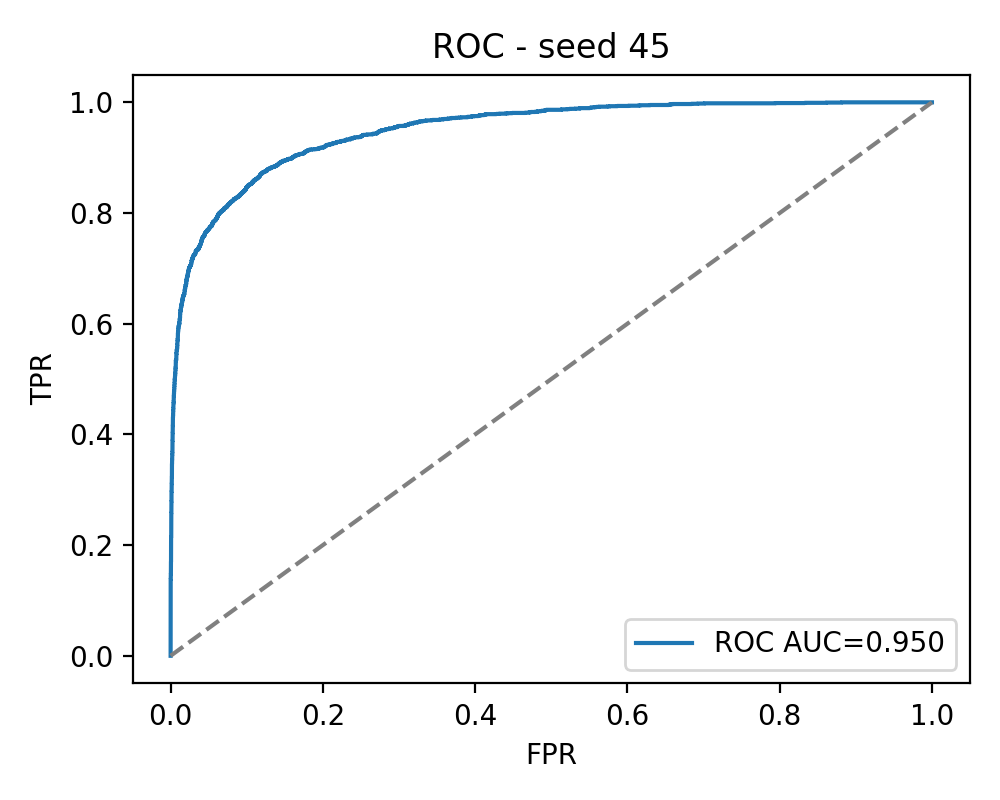
\includegraphics[width=.45\linewidth]{roc.png}
  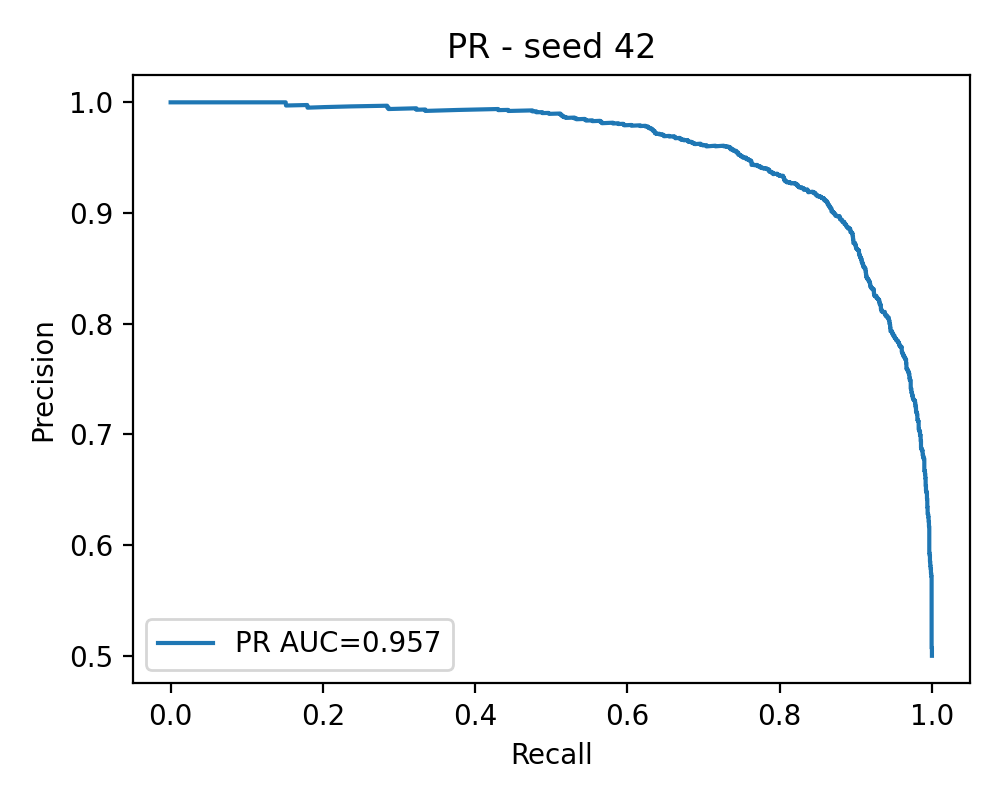
\includegraphics[width=.45\linewidth]{pr.png}
  \caption{ROC and PR curves for a representative seed.}
\end{figure}

\begin{figure}[H]
  \centering
  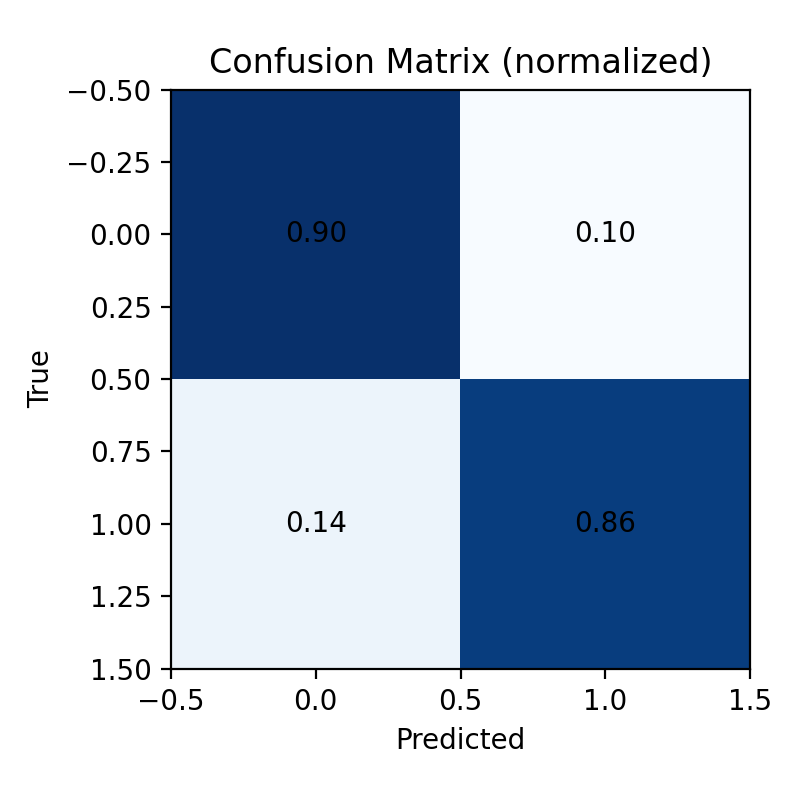
\includegraphics[width=.45\linewidth]{confusion.png}
  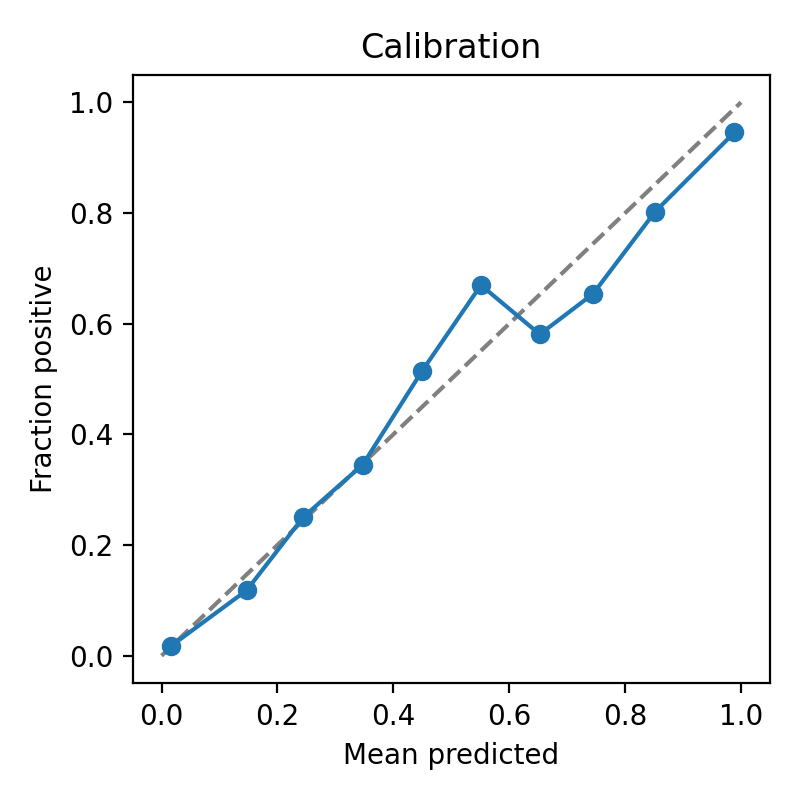
\includegraphics[width=.45\linewidth]{calibration.png}
  \caption{Confusion matrix (normalized) and calibration plot for a representative seed.}
\end{figure}

\noindent \textbf{Aggregate}: Table~\ref{tab:summary} summarizes the multi-seed test performance. Across five seeds, test accuracy averaged 0.8815 $\pm$ 0.0009 and ROC-AUC 0.9506 $\pm$ 0.0008, indicating strong discriminative performance with low variance across runs.

\begin{table}[H]
  \centering
  \caption{Multi-seed test performance (mean $\pm$ std) over 5 seeds.}
  \label{tab:summary}
  \begin{tabular}{lcc}
    \toprule
    Metric & Mean & Std \\
    \midrule
    Accuracy & 0.8815 & 0.0009 \\
    ROC-AUC  & 0.9506 & 0.0008 \\
    \bottomrule
  \end{tabular}
\end{table}

\noindent \textbf{Baseline Comparison}: Table~\ref{tab:baselines} compares our custom model against standard machine learning baselines on the same dataset using a 70/15/15 split. While our dual-branch architecture achieves the highest accuracy (88.1\%), F1-score (87.8\%), and ROC-AUC (95.1\%), the improvement over KNN is modest—only 1.7\% in accuracy and 2.4\% in ROC-AUC. XGBoost achieves higher precision (91.7\% vs 89.7\%) but significantly lower recall (73.9\% vs 86.0\%). The substantial gap between our model and simple baselines like logistic regression or SVMs suggests the task benefits from sequence-specific modeling, but the close performance with KNN indicates that complex architectures may not always be necessary for this dataset.

\begin{table}[H]
  \centering
  \caption{Model performance comparison on antimicrobial activity prediction task.}
  \label{tab:baselines}
  \begin{tabular}{lccccc}
    \toprule
    Model & Accuracy & Precision & Recall & F1-Score & ROC-AUC \\
    \midrule
    \textbf{My Model} & \textbf{88.1} & 89.7 & 86.0 & \textbf{87.8} & \textbf{95.1} \\
    KNN & 86.4 & 89.4 & 82.6 & 85.9 & 92.7 \\
    XGBoost & 83.6 & \textbf{91.7} & 73.9 & 81.8 & 91.0 \\
    Random Forest & 78.9 & 82.9 & 73.0 & 77.6 & 86.2 \\
    Logistic Regression & 50.6 & 50.3 & \textbf{87.1} & 63.8 & 49.7 \\
    SVM RBF & 53.0 & 52.1 & 72.6 & 60.7 & 50.6 \\
    SVM Linear & 49.2 & 49.2 & 50.2 & 49.7 & 52.8 \\
    \bottomrule
  \end{tabular}
\end{table}

\section{Discussion}
This project highlights both the strengths and limitations of combining automated code generation with domain expertise. As an individual with a background in machine learning, I was able to guide the model towards a working repository that successfully solved the expected problem. However, challenges remain, namely in dataset curation where the model was unable to develop a dataset for the task. While Claude accelerates boilerplate code generation and iteration, human expertise remains essential for curating data (thank you Nam Do), validating outputs, and interpreting results. 

\section{Next Steps}
Future work can extend to focusing on the 12\% holdouts that are not captured by the model. I propose conducting external tests against other datasets. Model improvements could focus on incorporating more data, orincluding transformer-based embeddings. 

\section{Conclusion}
I built a functional dataset and dual-branch predictor, established an evaluation that cements the success of the model at the task at hand. This provides a foundation for continued research and extensions.

\section*{References}
Nam Do (UC San Diego) who curating and shared the peptide–bacteria dataset used in this project.


\end{document}
